\documentclass[spanish,notitlepage,letterpaper,11pt]{article} % para artÌculo en castellano
\usepackage[utf8]{inputenc} % Acepta caracteres en castellano
\usepackage[T1]{fontenc} % font encoding
\usepackage[spanish]{babel} % silabea palabras castellanas
\usepackage[none]{hyphenat} 
\usepackage{amsmath}
\usepackage{amsfonts}
\usepackage{amssymb}
\usepackage[colorlinks=true,urlcolor=blue,linkcolor=blue]{hyperref} % navega por el doc
\usepackage{graphicx}
\usepackage{geometry} % See geometry.pdf to learn the layout options.
\geometry{letterpaper}  % ... or a4paper or a5paper or ... 
%\geometry{landscape}  % Activate for for rotated page geometry
%\usepackage[parfill]{parskip} % Activate to begin paragraphs with an empty line rather than an indent
\usepackage{epstopdf}
\usepackage{fancyhdr} % encabezados y pies de pg
\usepackage{lineno}
%\linenumbers

\pagestyle{fancy} 
\chead{\bfseries Aquí va el Título del documento} 
\lhead{} % si se omite coloca el nombre de la seccion
\rhead{fecha del doc} 
\lfoot{\it Autor  } 
\cfoot{Universidad Industrial de Santander} 
\rfoot{\thepage} 

\voffset = -0.25in 
\textheight = 8.0in 
\textwidth = 6.5in
\oddsidemargin = 0.in
\headheight = 20pt 
\headwidth = 6.5in
\renewcommand{\headrulewidth}{0.5pt}
\renewcommand{\footrulewidth}{0,5pt}
\DeclareGraphicsRule{.tif}{png}{.png}{`convert #1 `dirname #1`/`basename #1 .tif`.png}

\begin{document}
\title{Aquí va el Título del documento}
\author{
\textbf{Autor\thanks{e-mail: \texttt{autor@XXX.yyy.zz } }} \\ 
\textit{Nombre de Institución} \\ 
\textit{Dirección de la Institución}}
\date{Versión $\alpha \beta$ fecha del documento }
\maketitle
\tableofcontents
\begin{abstract}
El resumen debe ser suficiente para que uno no se lea el documento. Tiene que ser un articulito. Indicar frases telegráficas: la importancia de problema a estudiar (introducción), cómo se estudió (metodología), cuales fueron los resultados (Resultados) y cuál es la importancia de los resultados (conclusiones). Toda la información importante y trascendente del documento debe estar aquí. Típicamente debe tener una extensión entre 150 a 250 palabras.  
\end{abstract}

\section{Introducción}
Es el ?`Qué? del artículo. Aquí debe ir la descripción del problema, su importancia, sus antecedentes. Seguidamente, la justificación de este reporte, por qué se hace la investigación o reporta un caso, como se enmarca en los antecedentes y cuál es su importancia. Es importante, en la introducción resaltar los aportes de este trabajo con los antecedentes que los precedieron. Los acrónimos deben ser explicitados la primera vez que aparezcan.

La presentación de la introducción de lo general a lo particular. Se presente el contexto, su importancia, el problema y finalmente lo que abordará el artículo

Esta sección se finaliza con una descripción de lo que viene. Qué contienen cada una de las secciones.

\section{Metodología}
Es el ?`Cómo ? del artículo. En esta sección se echa el cuento de cómo se montó el experimento. La metodología experimental o teórica utilizada, sus detalles, haciendo referencia a los antecedentes. Cuáles herramientas (o técnicas) se utilizaron. El por qué se utilizaron: cuáles son las ventajas y las desventajas de esas herramientas. 

Esta sección tiene que garantizar la reproducibilidad del experimento o el cálculo

\subsection{Tablas}
Las Tablas deben ser lo más autocontenidas posibles. Sus títulos y  leyendas deben ser suficiente para explicar su contenido. Las tablas deben ser referidas desde el texto (ver Tabla \ref{Tabla1}). Si no se hace referencia a una tabla en particular, ésta se considera inútil para el artículo y debe ser suprimida

\begin{table}[h!]
  \centering
  \caption{Las leyendas se diferencia de las de la figuras en que van arriba de la Tabla. Deben explicar el contenido de las tablas. No ser meras descripciones de lo que se ve en las tablas. Deben generar reflexión respecto a lo que se quiere evidenciar en la tabla}  
\begin{tabular}{l|c|r}
\hline
% after \\ : \hline or \cline{col1-col2} \cline{col3-col4} ... este campo se usa para multicolumna
  Evento 1 & Evento 1  & Evento 3  \\ \hline
  Justificado Izquierdo & centrado & Justificado derecho \\ 
   &  &  \\ \hline \hline
\hline
\end{tabular}   
  \label{Tabla1}
\end{table}


\section{El experimento y los resultados}
¿Qué se midió? ¿cuáles fueron las condiciones de medición? ¿que representan esas medidas? ¿cuáles son las limitaciones de la medida por las restricciones que impone la técnica y las herramientas?

¿Cuáles fueron los resultados? Incluyendo algunos comentarios y discusiones que serán reforzadas en las conclusiones. 


\subsection{Figuras}
Al igual que las Tablas, las Figuras deben ser lo mas autocontenidas posibles. Sus títulos y  leyendas deben ser suficiente para explicar su contenido. Las figuras deben ser referidas desde el texto (ver Figura (o Fig) \ref{Figura1}). Otra vez, si no se hace referencia a una figura en particular, ésta se considera inútil para el artículo y debe ser suprimida

\begin{figure}
\begin{center}
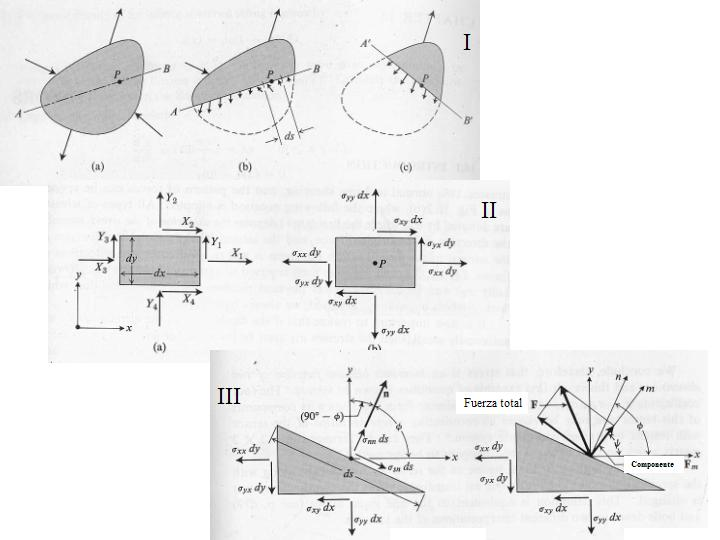
\includegraphics[width=4in]{FigModeloReporte/FigTensorEsfuerzos2D.jpg}
\caption{Esta figura incorpora una imagen}
\label{Figura1}
\end{center}
\end{figure}


\section{Conclusiones y Recomendaciones}
A partir de las medidas ¿qué se concluyó? ¿cuál fue el aporte de este esfuerzo? ¿qué se recomienda hacer? ¿cuáles serían los próximos pasos o acciones a tomar? 

La estructura de las conclusiones es invertida a la de la introducción. Comienza explicitando/enumerando los principales resultados. Luego sigue una interpretación de esos resultados y finaliza con la trascendencia de los resultados.  

Quizá la mejor recomendación es consultar el libro de Umberto de Cómo hacer una Tesis Doctoral\cite{Eco1986} \footnote{\url{http://web.usal.es/~mom/tesis_eco.pdf}}. 

Otra posible fuente de información puede ser el libro de \textit{A guide to Effective Publishing in Astronomy} \cite{BertoutBiemesderferHenri2012} donde además aparece reseñado todo el proceso de publicación en Astronomía. 
\footnote{\url{https://astro.mff.cuni.cz/vyuka/AST031/guide.pdf}}


\section{Referencias}
Aquí deben ir las referencias citadas \cite{Narasimhan1993} cuando corresponda y los url que se consideren necesarios y que hayan sido citadas en el texto del documento. Es mucho más fácil utilizar \texttt{Bibtex}, que es un mecanismo para citar referencias siguiendo los patrones internacionales. Si no se hace uso de \texttt{Bibtex} se tiene que tener cuidado de citar de la forma que lo requiera la publicación. Si no hay recomendaciones de los editores, lo mejor es apegarse a algún estilo estándar y civilizado de presentar la bibliografía Hay muchos por allí \url{http://www.researchconsultation.com/dissertation-references-thesis-citations-bibliography.asp}. 

\bibliographystyle{unsrt}
\bibliography{BibTex/BiblioLN130519}

%\begin{thebibliography}{99}
%\bibitem{Narasimhan1993}Narasimhan, M.N.L., (1993), \textit{Principles of
%Continuum Mechanics}, (John Willey, New York) p. 510.

%\bibitem{Demianski1985}Demia\'{n}ski M., (1985), \textit{Relativistic
%Astrophysics,} in International Series in Natural Philosophy, Vol 110, Edited
%by \textit{D. Ter Haar}, (Pergamon Press, Oxford).
%\end{thebibliography}

\end{document}  